\documentclass[12pt]{article}

% ── Page geometry ────────────────────────────────────────────────────────────
\usepackage[a4paper, margin=1in]{geometry}
\usepackage{setspace}
\singlespacing

% ── Fonts & encoding ────────────────────────────────────────────────────────
\usepackage[T1]{fontenc}
\usepackage[utf8]{inputenc}
\usepackage{lmodern}

% ── Packages ─────────────────────────────────────────────────────────────────
\usepackage{graphicx}
\usepackage{booktabs}
\usepackage{multirow}
\usepackage{amsmath, amssymb}
\usepackage{hyperref}
\usepackage{xcolor}
\usepackage{enumitem}
\usepackage{caption}
\usepackage{subcaption}
\usepackage{float}
\usepackage{listings}
\usepackage{xurl}

\hypersetup{
    colorlinks=true,
    linkcolor=blue!70!black,
    citecolor=blue!70!black,
    urlcolor=blue!70!black,
}

\captionsetup{font={small}, labelfont={bf}}

% ── Code listing style ──────────────────────────────────────────────────────
\lstset{
    language=Python,
    basicstyle=\ttfamily\scriptsize,
    keywordstyle=\color{blue!70!black}\bfseries,
    commentstyle=\color{green!50!black}\itshape,
    stringstyle=\color{red!60!black},
    numbers=left,
    numberstyle=\tiny\color{gray},
    numbersep=5pt,
    frame=single,
    framesep=3pt,
    breaklines=true,
    breakatwhitespace=false,
    showstringspaces=false,
    tabsize=4,
    captionpos=b,
    xleftmargin=1.5em,
    framexleftmargin=1.5em,
}

% ── Title ────────────────────────────────────────────────────────────────────
\title{
    \textbf{Corporate Evasion Decoder: Detecting Evasive Communication in
    Earnings Call Q\&A Sessions}
}
\author{
    Wei-Lin Wen (Student ID: 314551086)\\[2pt]
    National Yang Ming Chiao Tung University
}
\date{}

% ═════════════════════════════════════════════════════════════════════════════
\begin{document}
\maketitle
\thispagestyle{empty}

\noindent\textbf{Dataset Repository:}
\url{https://github.com/weilin1205/CorporateEvasionDecoder}

% ─────────────────────────────────────────────────────────────────────────────
\section{Research Question and Motivation}
% ─────────────────────────────────────────────────────────────────────────────

Corporate earnings calls are a primary channel through which public companies
communicate financial performance to investors and analysts. During the Q\&A
portion, executives may respond with varying degrees of transparency: some
answers are direct and data-driven, while others employ hedging language,
excessive jargon, or strategic vagueness to deflect difficult questions.
Detecting such evasive communication is valuable for financial analysts,
regulators, and NLP researchers.

I pose the following research question: \emph{Can I automatically classify
corporate Q\&A responses as \textsc{Direct}, \textsc{Evasive}, or
\textsc{Jargon}-heavy using a combination of handcrafted linguistic features
and text representations?}

This task is challenging because evasiveness is subjective, corporate
jargon is domain-specific, and the dataset is modest ($n = 1{,}129$),
making high-capacity models prone to overfitting---an ideal testbed
for comparing classical ML against a fine-tuned transformer.

% ─────────────────────────────────────────────────────────────────────────────
\section{Dataset Documentation}
% ─────────────────────────────────────────────────────────────────────────────

\subsection{Data Type and Source}

Each sample is a \textbf{question--answer pair} extracted from public earnings
call transcripts. The text is in English and drawn from formal corporate
communication. Transcripts were obtained from \textbf{SeekingAlpha}
via the RapidAPI endpoint
\texttt{seeking-alpha.p.rapidapi.com}~\cite{seekingalpha}.

\subsection{Amount and Composition}

\begin{table}[htbp]
\centering
\caption{Dataset composition by label and sector.}
\label{tab:composition}
\begin{tabular*}{\linewidth}{@{\extracolsep{\fill}} ll}
  % ── Left sub-table: Class distribution ──────────────────────────────
  \begin{minipage}[t]{0.42\linewidth}
    \centering
    \captionof*{table}{(a) Class distribution.}
    \small
    \begin{tabular}{lrr}
      \toprule
      \textbf{Label} & \textbf{Count} & \textbf{Prop.} \\
      \midrule
      \textsc{Direct}  & 395 & 35.0\% \\
      \textsc{Evasive} & 352 & 31.2\% \\
      \textsc{Jargon}  & 382 & 33.8\% \\
      \midrule
      \textbf{Total}   & 1{,}129 & 100.0\% \\
      \bottomrule
    \end{tabular}
    \label{tab:class_dist}
  \end{minipage}
  &
  % ── Right sub-table: Sector distribution ────────────────────────────
  \begin{minipage}[t]{0.54\linewidth}
    \centering
    \captionof*{table}{(b) Sector distribution.}
    \footnotesize
    \begin{tabular}{l p{5.1cm} r}
      \toprule
      \textbf{Sector} & \textbf{Tickers} & \textbf{\#} \\
      \midrule
      Technology  & AAPL, MSFT, GOOGL, META, AMZN, NVDA & 6 \\
      Finance     & JPM, GS, BAC          & 3 \\
      Healthcare  & JNJ, PFE, UNH         & 3 \\
      Consumer    & PG, KO, WMT, MCD      & 4 \\
      Energy      & XOM, CVX              & 2 \\
      Industrial  & CAT, GE               & 2 \\
      \midrule
      \textbf{Total} & & \textbf{20} \\
      \bottomrule
    \end{tabular}
  \end{minipage}
\end{tabular*}
\end{table}

The dataset spans \textbf{20 companies} across \textbf{6 sectors}
(Table~\ref{tab:composition}). A total of 131 transcripts were crawled,
of which 87 contained extractable Q\&A sections, yielding 1{,}129 pairs
with a well-balanced class distribution ($\approx$33\% each).

\subsection{Collection Process}

Data collection followed a four-stage pipeline:
\begin{enumerate}[nosep]
    \item \textbf{Crawling.} For each of the 20 tickers, up to 8 recent
          earnings call transcript IDs were retrieved via the SeekingAlpha API.
          Full HTML transcripts were then downloaded (131 total, capped at
          480 API calls).
    \item \textbf{Q\&A extraction.} HTML transcripts were parsed to isolate
          the Q\&A section. Speaker turns were segmented by
          \texttt{<p>} tags with speaker-name formatting. Analyst questions
          were paired with the subsequent executive answer, yielding
          structured \texttt{(question, answer, ticker, date)} tuples.
    \item \textbf{LLM annotation.} Each Q\&A pair was classified by
          \textbf{Qwen3.5-9B}~\cite{qwen} running locally on an
          NVIDIA RTX A6000 GPU with zero-shot
          prompting. The prompt asked the model to assign exactly one of
          three labels---\textsc{Direct}, \textsc{Evasive}, or
          \textsc{Jargon}---based on explicit criteria (e.g., hedging
          language, numerical specificity, buzzword density). This
          semi-automatic approach enabled labeling the full dataset
          consistently while acknowledging that label noise is inevitable.
    \item \textbf{Feature engineering.} Two feature families were computed:
          500-dimensional TF-IDF vectors (unigrams + bigrams) and 21
          handcrafted linguistic features (see Section~\ref{sec:features}).
\end{enumerate}

\subsection{Conditions and Limitations}

Transcripts are public, sourced from a commercial API, and contain no
personally identifiable information beyond public executive names. The
LLM-generated labels introduce systematic noise: the annotator has no
ground-truth human labels for calibration. I acknowledge this as the
primary limitation and discuss its impact on model performance in
Section~\ref{sec:discussion}.

\subsection{Examples}

\begin{itemize}[nosep]
    \item \textbf{Direct:} \emph{``Revenue grew 12\% year-over-year to
          \$23.4 billion, driven primarily by cloud services which grew
          28\%.''}
    \item \textbf{Evasive:} \emph{``I continue to evaluate our strategic
          options and remain focused on long-term value creation for our
          stakeholders across the portfolio.''}
    \item \textbf{Jargon:} \emph{``We're leveraging our synergistic
          ecosystem to drive paradigm-shifting innovation across
          verticals.''}
\end{itemize}

% ─────────────────────────────────────────────────────────────────────────────
\section{Feature Engineering}
\label{sec:features}
% ─────────────────────────────────────────────────────────────────────────────

The feature space comprises \textbf{521 dimensions}: 500 TF-IDF features and
21 handcrafted linguistic features designed to capture communication style
beyond bag-of-words statistics.

\begin{table}[H]
\centering
\caption{The 21 handcrafted linguistic features grouped by category.}
\label{tab:features}
\small
\begin{tabular}{llp{6.5cm}}
\toprule
\textbf{Category} & \textbf{Feature} & \textbf{Description} \\
\midrule
\multirow{5}{*}{Length}
    & \texttt{answer\_word\_count}      & Word count of the answer \\
    & \texttt{answer\_sent\_count}      & Sentence count of the answer \\
    & \texttt{avg\_sent\_length}        & Average sentence length (words) \\
    & \texttt{question\_word\_count}    & Word count of the question \\
    & \texttt{qa\_length\_ratio}        & Answer length / question length \\
\midrule
\multirow{2}{*}{Hedging}
    & \texttt{hedge\_word\_count}       & Count of hedge words (\emph{might, could, possibly, generally}, etc.) \\
    & \texttt{hedge\_word\_ratio}       & Proportion of hedge words \\
\midrule
\multirow{2}{*}{Jargon}
    & \texttt{jargon\_word\_count}      & Count of corporate jargon (\emph{synergy, leverage, ecosystem}, etc.) \\
    & \texttt{jargon\_word\_ratio}      & Proportion of jargon words \\
\midrule
\multirow{4}{*}{Specificity}
    & \texttt{number\_count}            & Count of numeric tokens \\
    & \texttt{number\_ratio}            & Proportion of numeric tokens \\
    & \texttt{metric\_count}            & Count of metric phrases (e.g., \emph{\$X billion}) \\
    & \texttt{metric\_ratio}            & Proportion of metric phrases \\
\midrule
\multirow{2}{*}{Pronouns}
    & \texttt{first\_person\_ratio}     & Ratio of first-person pronouns \\
    & \texttt{third\_person\_ratio}     & Ratio of third-person pronouns \\
\midrule
\multirow{2}{*}{Complexity}
    & \texttt{avg\_word\_length}        & Average word length (characters) \\
    & \texttt{long\_word\_ratio}        & Proportion of words $\geq 7$ characters \\
\midrule
\multirow{2}{*}{Structure}
    & \texttt{starts\_with\_direct\_answer} & Binary: starts with yes/no/number \\
    & \texttt{question\_keyword\_overlap}   & Jaccard overlap of Q\&A keywords \\
\midrule
Semantic
    & \texttt{qa\_tfidf\_similarity}    & Cosine similarity between Q\&A TF-IDF vectors \\
\bottomrule
\end{tabular}
\end{table}

The TF-IDF~\cite{tfidf} features were extracted from the concatenated
question--answer text using scikit-learn's \texttt{TfidfVectorizer}~\cite{sklearn}
with a maximum of 500 features (unigrams and bigrams). The handcrafted features
capture stylistic and structural properties that are hypothesized to
discriminate between direct, evasive, and jargon-heavy responses.

% ─────────────────────────────────────────────────────────────────────────────
\section{Methods}
\label{sec:methods}
% ─────────────────────────────────────────────────────────────────────────────

I evaluate four classifiers spanning a spectrum from linear models to
deep pre-trained transformers. All classical models use the full 521-feature
representation; DistilBERT operates on raw text.

\paragraph{Logistic Regression (LR).}
Multinomial LR with L2 regularization ($C = 1.0$, L-BFGS solver).
Serves as a transparent linear baseline with interpretable coefficients.

\paragraph{Support Vector Machine (SVM).}
RBF-kernel SVM ($C = 1.0$, $\gamma = \text{scale}$) with one-vs-rest
decomposition and Platt scaling for probability estimates.

\paragraph{XGBoost.}
Gradient-boosted trees~\cite{xgboost}: 100 estimators, depth 4,
learning rate 0.1. Built-in gain-based feature importance is used for
ablation analysis.

\paragraph{DistilBERT.}
Fine-tuned \texttt{distilbert-base-uncased}~\cite{distilbert} via
Hugging Face Transformers~\cite{transformers} with a linear head,
class-weighted cross-entropy loss, learning rate $5\!\times\!10^{-5}$,
dropout 0.3, and early stopping (patience 3, up to 10 epochs).

\paragraph{Evaluation Protocol.}
All models were evaluated using \textbf{stratified 5-fold cross-validation}
to ensure each fold preserves the class distribution. I report
accuracy, macro-averaged F1 score, and one-vs-rest AUROC.
Per-class precision, recall, and F1 are reported for detailed analysis.

% ─────────────────────────────────────────────────────────────────────────────
\section{Experiments and Results}
\label{sec:experiments}
% ─────────────────────────────────────────────────────────────────────────────

\subsection{Experiment 1: Baseline Comparison}

Table~\ref{tab:baseline} presents the baseline performance of all four
models on the full 521-feature set (or raw text for DistilBERT).

\begin{table*}[htbp]
\centering
\small
\begin{minipage}[t]{0.7\linewidth}
  \centering
  \captionof{table}{Baseline 5-fold cross-validation results (mean $\pm$ std).}
  \label{tab:baseline}
  \resizebox{\linewidth}{!}{%
    \begin{tabular}{lccc}
      \toprule
      \textbf{Model} & \textbf{Accuracy} & \textbf{F1 (macro)} & \textbf{AUROC} \\
      \midrule
      Logistic Regression & $0.455 \pm 0.027$ & $0.453 \pm 0.026$ & 0.646 \\
      SVM (RBF)           & $0.532 \pm 0.037$ & $0.528 \pm 0.036$ & 0.731 \\
      XGBoost             & $0.544 \pm 0.029$ & $0.542 \pm 0.030$ & 0.728 \\
      DistilBERT          & $\mathbf{0.582 \pm 0.031}$ & $\mathbf{0.580 \pm 0.031}$ & $\mathbf{0.745 \pm 0.031}$ \\
      \bottomrule
    \end{tabular}%
  }
\end{minipage}
\end{table*}

\begin{table}[htbp]
\centering
\caption{Per-class precision, recall, and F1 for all classical models (5-fold CV averages).}
\label{tab:perclass}
\small
\begin{tabular}{llccc}
\toprule
\textbf{Model} & \textbf{Class} & \textbf{Precision} & \textbf{Recall} & \textbf{F1} \\
\midrule
\multirow{3}{*}{Logistic Regression}
  & \textsc{Direct}  & 0.520 & 0.524 & 0.522 \\
  & \textsc{Evasive} & 0.411 & 0.423 & 0.417 \\
  & \textsc{Jargon}  & 0.427 & 0.411 & 0.419 \\
\midrule
\multirow{3}{*}{SVM (RBF)}
  & \textsc{Direct}  & 0.580 & 0.595 & 0.588 \\
  & \textsc{Evasive} & 0.514 & 0.480 & 0.496 \\
  & \textsc{Jargon}  & 0.496 & 0.513 & 0.505 \\
\midrule
\multirow{3}{*}{XGBoost}
  & \textsc{Direct}  & 0.571 & 0.603 & 0.586 \\
  & \textsc{Evasive} & 0.541 & 0.509 & 0.524 \\
  & \textsc{Jargon}  & 0.517 & 0.516 & 0.516 \\
\bottomrule
\end{tabular}
\end{table}

DistilBERT achieves the highest performance, demonstrating that
pre-trained contextual representations provide an advantage over
handcrafted features for this task. Among classical models, XGBoost leads
marginally over SVM, while Logistic Regression lags substantially.

Table~\ref{tab:perclass} breaks down per-class performance across all
classical models. \textsc{Direct} is consistently the easiest class
(F1 $\approx$ 0.59), while \textsc{Evasive} and \textsc{Jargon} overlap
significantly (F1 $\approx$ 0.50--0.52).

\begin{figure}[H]
    \centering
    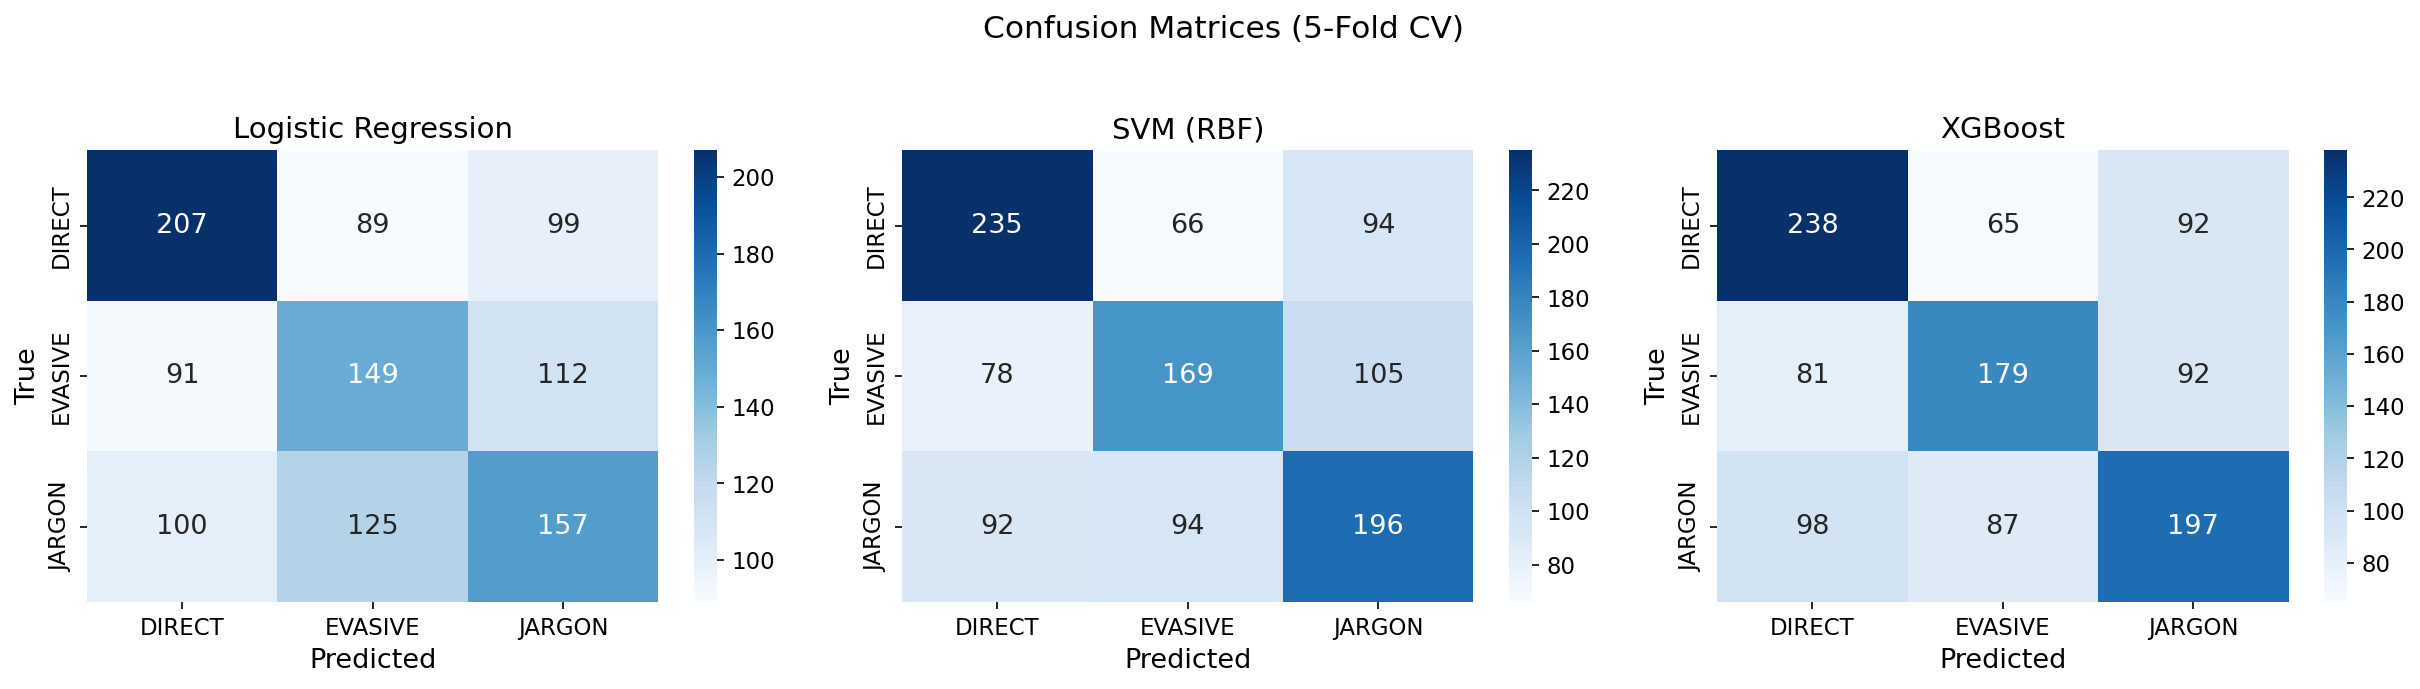
\includegraphics[width=1\linewidth]{figures/fig_confusion_matrices.png}
    \caption{Confusion matrices for classical models.}
    \label{fig:confusion}
\end{figure}

\begin{figure}[htbp]
    \centering
    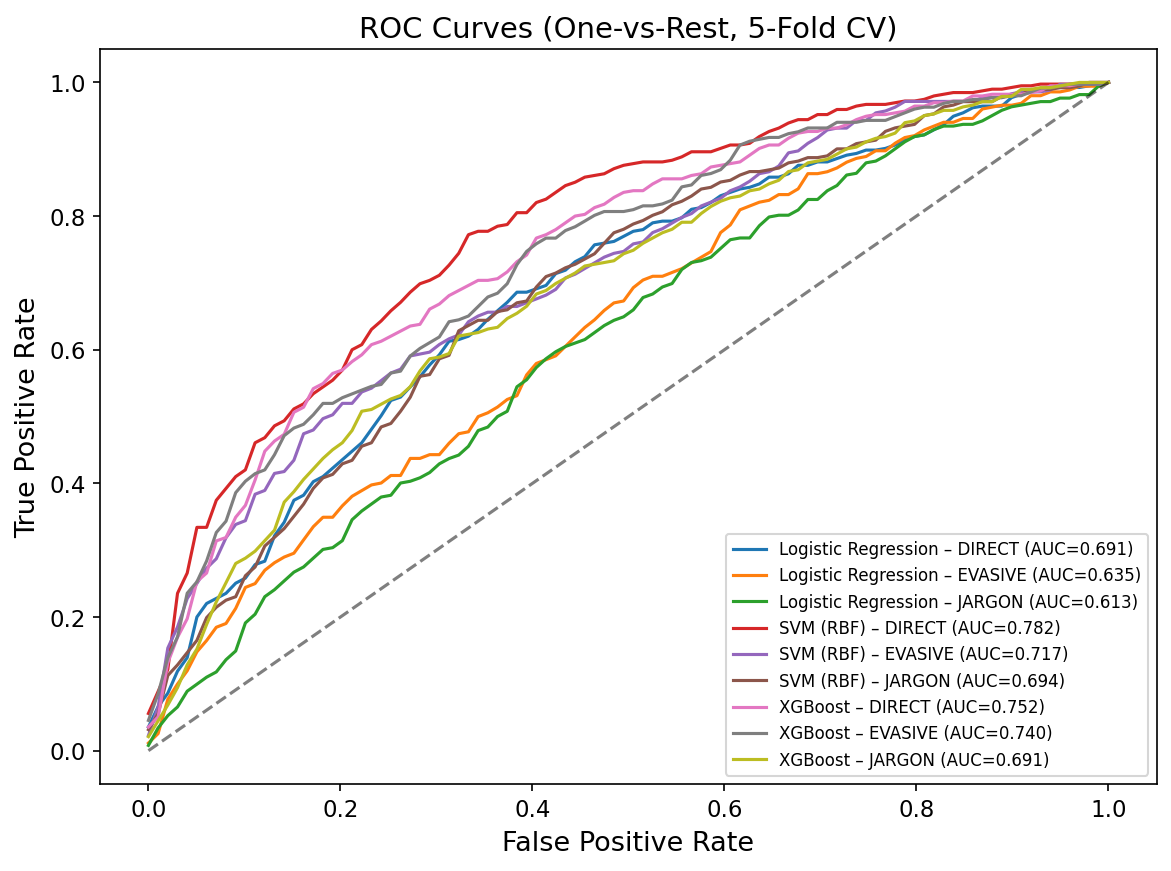
\includegraphics[width=0.65\linewidth]{figures/fig_roc_curves.png}
    \caption{One-vs-rest ROC curves.}
     \label{fig:roc}
\end{figure}

The confusion matrices (Figure~\ref{fig:confusion}) reveal that
\textsc{Evasive} and \textsc{Jargon} are frequently confused with each
other, consistent with our intuition that both involve non-specific,
non-committal language. The ROC curves (Figure~\ref{fig:roc}) show that
all models achieve AUROC well above 0.5 for each class, confirming that
the features carry discriminative signal despite the modest overall accuracy.

% ── Experiment 2 ─────────────────────────────────────────────────────────────
\subsection{Experiment 2: Learning Curves}

\begin{figure}[htbp]
    \centering
    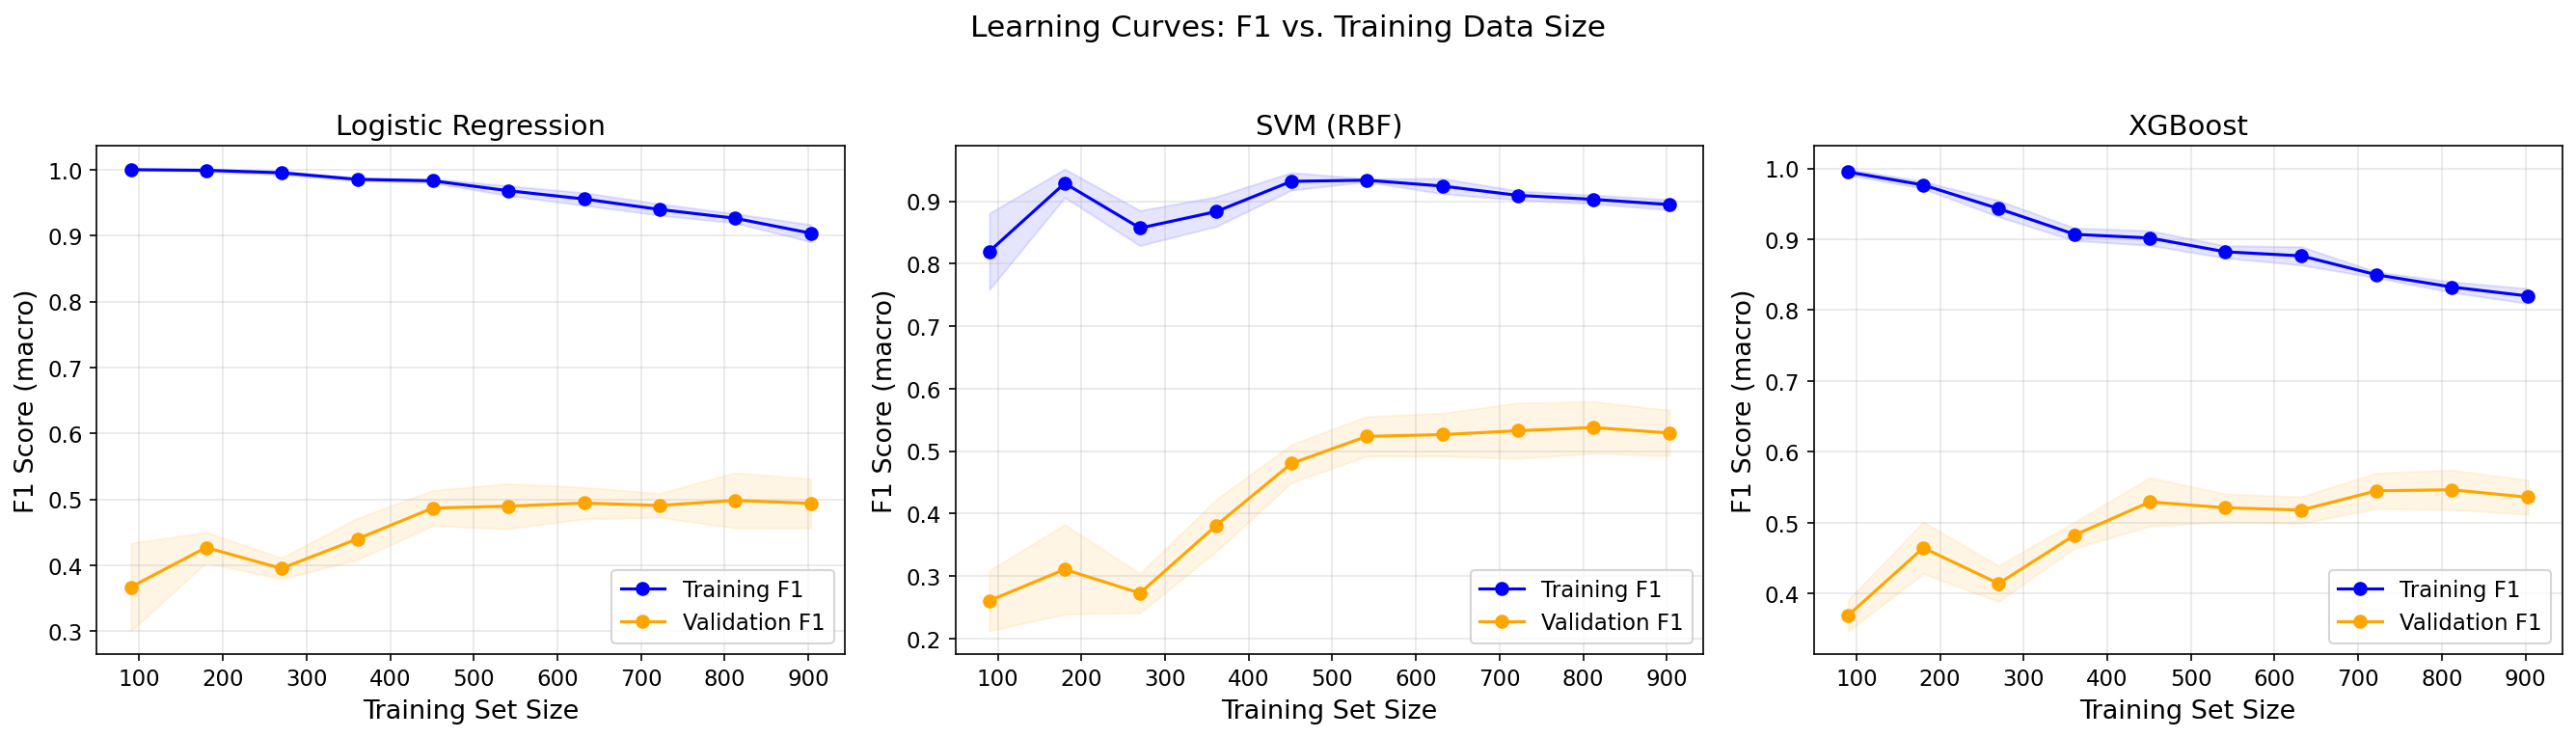
\includegraphics[width=1.0\textwidth]{figures/fig_learning_curves.png}
    \caption{Learning curves showing training vs.\ validation F1 as a
             function of training set fraction.}
    \label{fig:learning}
\end{figure}

Figure~\ref{fig:learning} shows that all models exhibit a persistent
training--validation gap, indicating overfitting. Validation F1 improves
as more data is added but plateaus around 0.55, suggesting that
performance is bounded not only by model capacity but also by label noise
from the LLM annotator. The upward trend at larger training fractions
indicates that \emph{more data would likely help}; this hypothesis is
confirmed by the LLM data augmentation experiment (Section~\ref{sec:augment}),
which yields 10--12 F1-point gains.

% ── Experiment 3 ─────────────────────────────────────────────────────────────
\subsection{Experiment 3: SMOTE Analysis}

Since class imbalance can degrade minority-class performance, I evaluated
SMOTE~\cite{smote} (Synthetic Minority Oversampling Technique) applied
within each cross-validation fold.

\begin{table}[htbp]
\centering
\caption{Effect of SMOTE on macro-F1.}
\label{tab:smote}
\small
\begin{tabular}{lccc}
\toprule
\textbf{Model} & \textbf{No SMOTE} & \textbf{With SMOTE} & \textbf{$\Delta$} \\
\midrule
Logistic Regression & 0.453 & 0.453 & $-0.000$ \\
SVM (RBF)           & 0.528 & 0.523 & $-0.005$ \\
XGBoost             & 0.542 & 0.546 & $+0.004$ \\
\bottomrule
\end{tabular}
\end{table}

\begin{figure}[H]
    \centering
    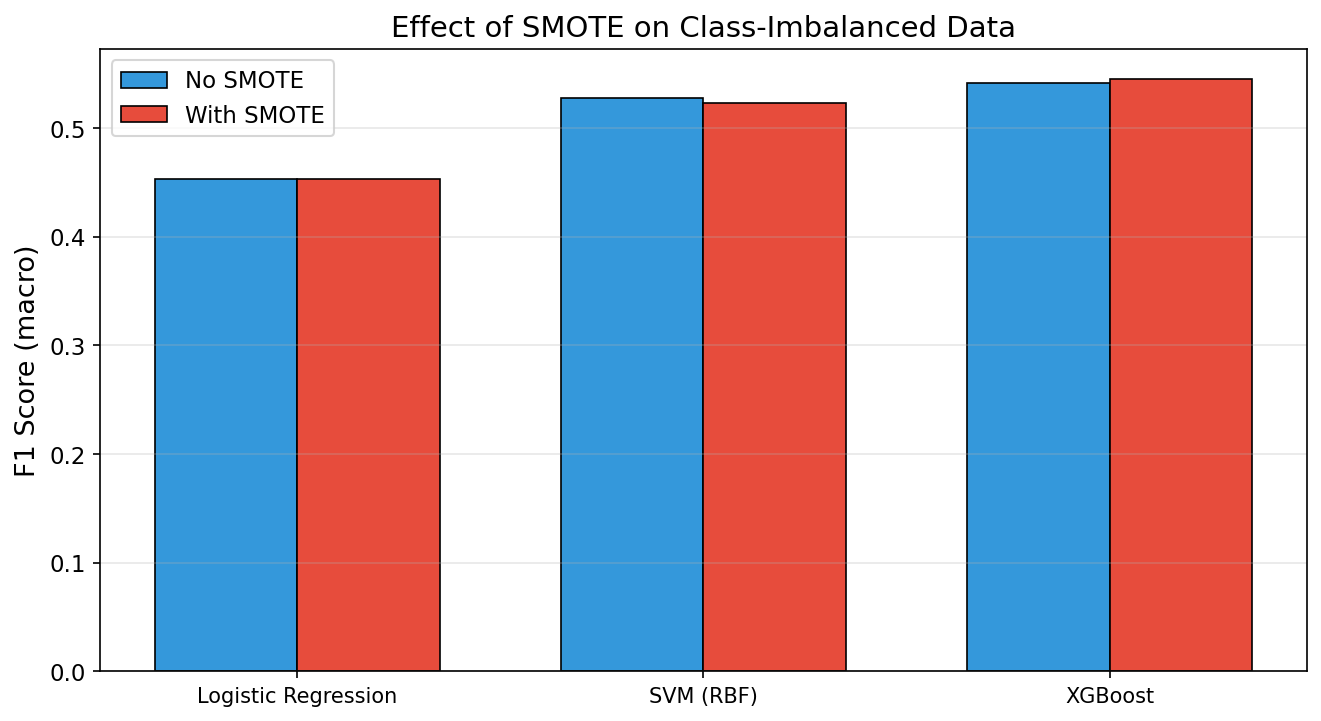
\includegraphics[width=0.55\textwidth]{figures/fig_smote_comparison.png}
    \caption{SMOTE vs.\ no-SMOTE comparison across models.}
    \label{fig:smote}
\end{figure}

SMOTE produces negligible changes ($|\Delta| < 0.006$) for all models.
This is expected: the dataset is already well-balanced (35/31/34\%), so
oversampling the slightly smaller \textsc{Evasive} class adds little
value. For SVM, the synthetic samples even introduce a slight performance
drop, possibly because SMOTE-generated points near the decision boundary
add noise in high-dimensional feature space. This experiment confirms
that class imbalance is \emph{not} a contributing factor to the moderate
accuracy.

% ── Experiment 4 ─────────────────────────────────────────────────────────────
\subsection{Experiment 4: PCA Dimensionality Reduction}

With 521 features and only 1{,}129 samples, the curse of dimensionality
may harm linear models. I applied PCA to the feature matrix and evaluated
performance at various component counts.

\begin{table}[H]
\centering
\caption{Macro-F1 as a function of PCA components.}
\label{tab:pca}
\small
\begin{tabular}{lccc}
\toprule
\textbf{Components} & \textbf{LR} & \textbf{SVM} & \textbf{XGBoost} \\
\midrule
25              & 0.538          & 0.528          & 0.513          \\
50              & \textbf{0.545} & \textbf{0.534} & 0.529          \\
100             & 0.519          & 0.527          & 0.516          \\
200             & 0.497          & 0.524          & 0.509          \\
521 (full)      & 0.453          & 0.528          & \textbf{0.542} \\
\bottomrule
\end{tabular}
\end{table}

\begin{figure}[htbp]
    \centering
    \begin{minipage}[t]{0.48\textwidth}
        \centering
        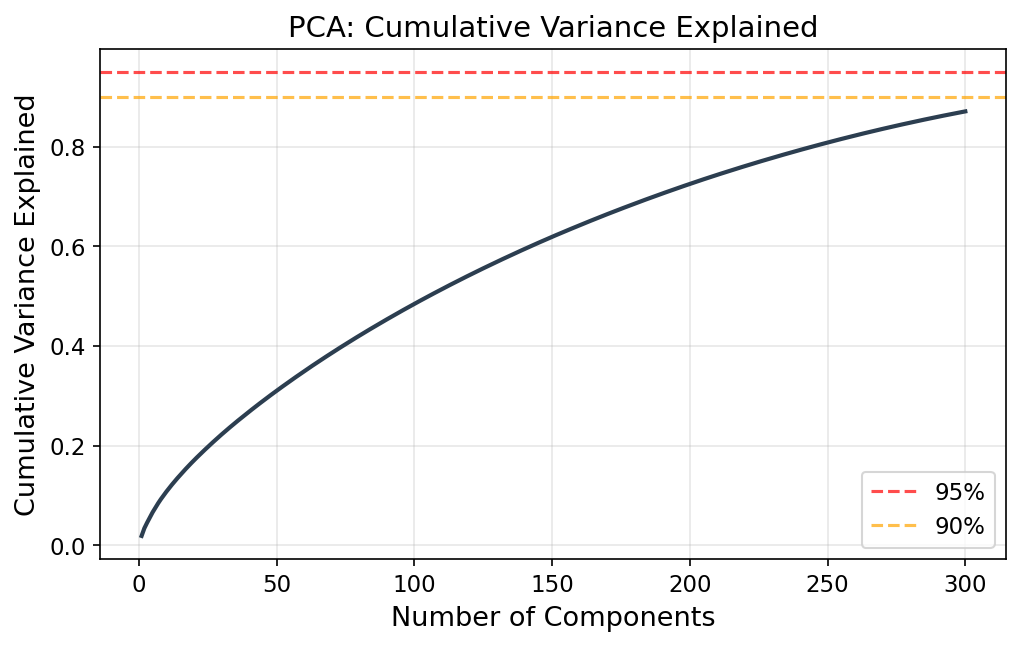
\includegraphics[width=\textwidth]{figures/fig_pca_variance.png}
        \caption{Cumulative explained variance by PCA.}
        \label{fig:pca_var}
    \end{minipage}
    \hfill
    \begin{minipage}[t]{0.48\textwidth}
        \centering
        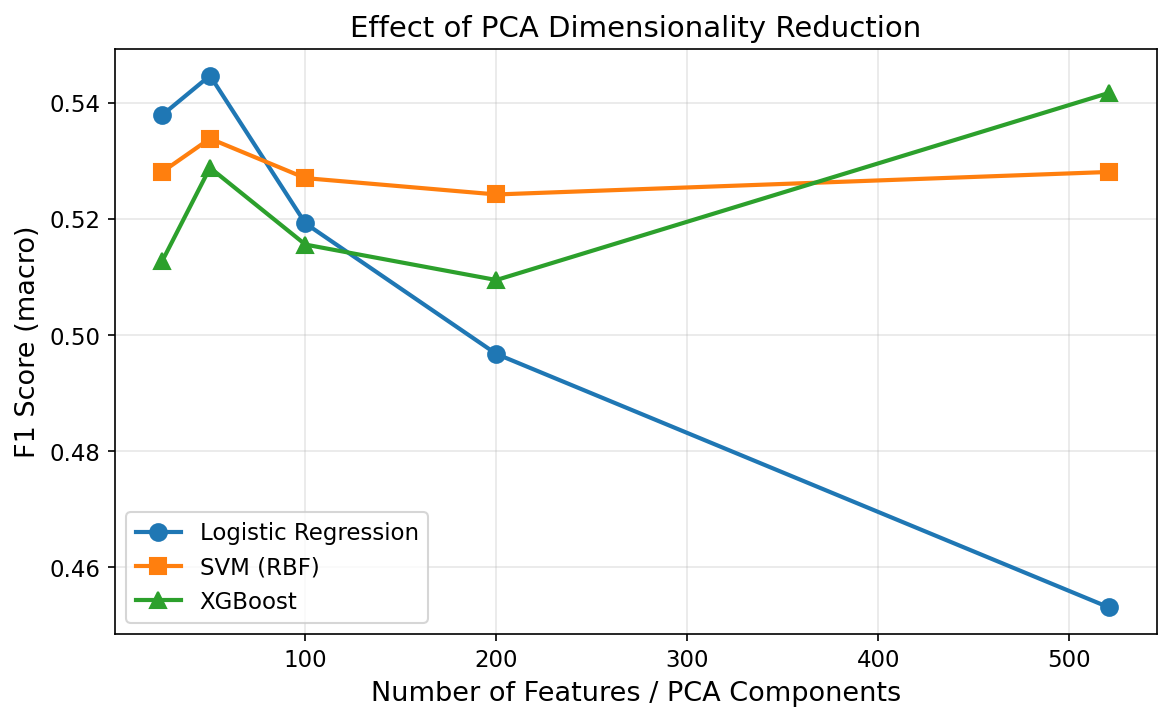
\includegraphics[width=\textwidth]{figures/fig_pca_performance.png}
        \caption{Model performance vs.\ PCA components.}
        \label{fig:pca_perf}
    \end{minipage}
\end{figure}

The key finding is that \textbf{PCA-50 dramatically improves Logistic
Regression} from F1 = 0.453 to 0.545 (+20\%), making it competitive with
SVM and XGBoost. This reveals that LR's poor baseline performance stems
not from insufficient model capacity but from overfitting to
high-dimensional noise. PCA acts as a regularizer by projecting out
low-variance (likely noisy) directions.

SVM is relatively robust across dimensionalities, consistent with the
RBF kernel's implicit regularization through $\gamma = \text{scale}$.
XGBoost performs best with all 521 features because its tree-based
structure performs built-in feature selection by only splitting on
informative features.

% ── Experiment 5 ─────────────────────────────────────────────────────────────
\subsection{Experiment 5: Feature Ablation}

To quantify the contribution of each feature family, I compared
TF-IDF--only, handcrafted--only, and combined feature sets.

\begin{table}[htbp]
\centering
\caption{Feature ablation: macro-F1 by feature subset.}
\label{tab:ablation}
\small
\begin{tabular}{lccc}
\toprule
\textbf{Feature Set} & \textbf{LR} & \textbf{SVM} & \textbf{XGBoost} \\
\midrule
TF-IDF Only (500)        & 0.439          & 0.510          & 0.508          \\
Handcrafted Only (21)     & \textbf{0.518} & 0.511          & 0.513          \\
Combined (521)            & 0.453          & 0.528          & \textbf{0.542} \\
\bottomrule
\end{tabular}
\end{table}

The most striking result is that \textbf{21 handcrafted features
outperform 500 TF-IDF features} for Logistic Regression (0.518 vs.\ 0.439)
and match SVM performance (0.511 vs.\ 0.510). This underscores the value
of domain-informed feature engineering: the handcrafted features distill
the linguistically relevant signal into a compact, low-noise
representation that linear models can exploit effectively.

For XGBoost, combining both feature families yields the best result
(0.542), suggesting that the ensemble learner benefits from both the
fine-grained lexical signal in TF-IDF and the high-level stylistic
signal in handcrafted features. The tree-based model can selectively
attend to informative features from either family while ignoring noise.

\begin{figure}[htbp]
    \centering
    \begin{minipage}[t]{0.48\textwidth}
        \centering
        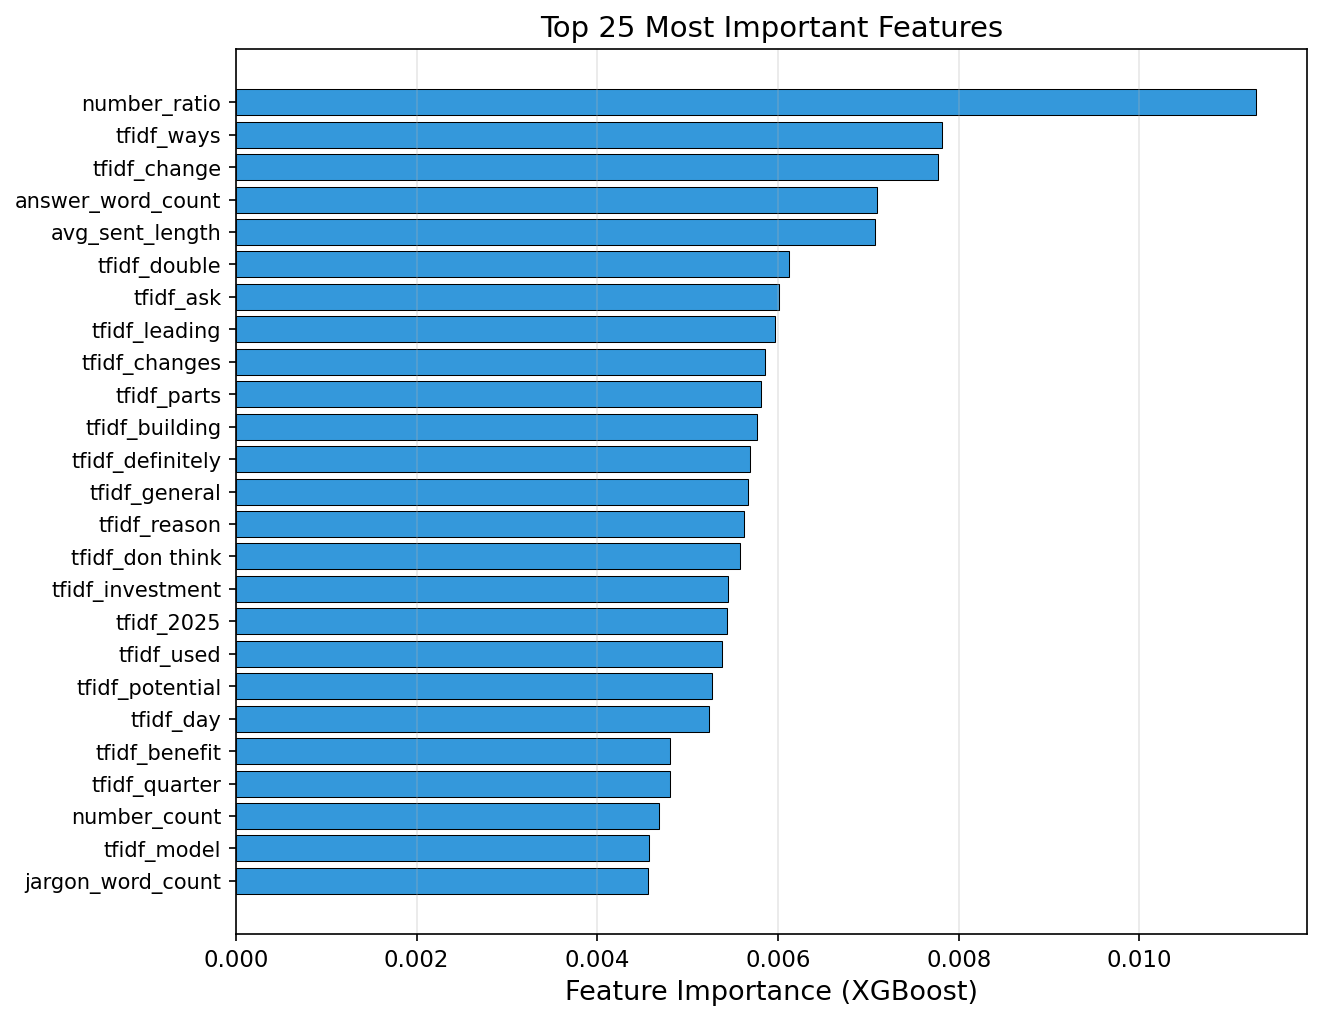
\includegraphics[width=\textwidth]{figures/fig_feature_importance.png}
        \caption{Top features by XGBoost gain (full set).}
        \label{fig:feat_imp}
    \end{minipage}
    \hfill
    \begin{minipage}[t]{0.48\textwidth}
        \centering
        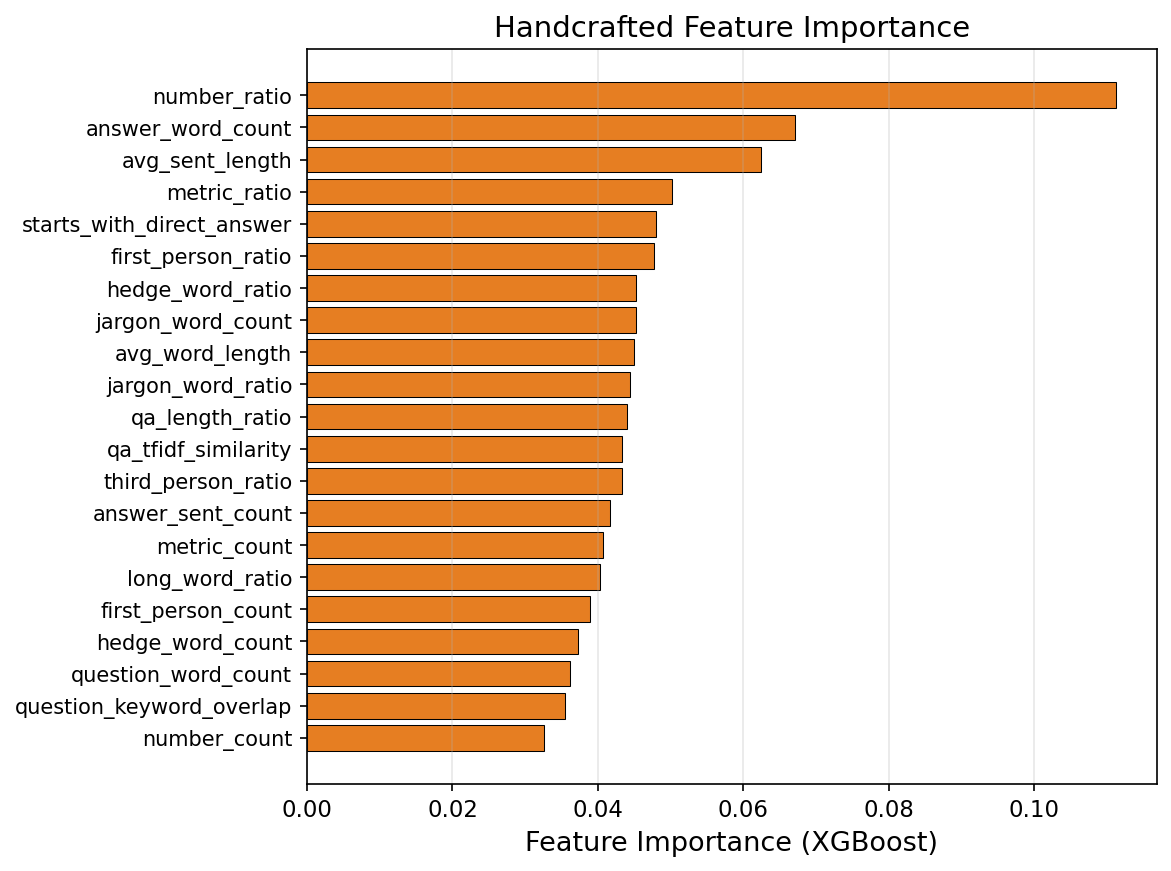
\includegraphics[width=\textwidth]{figures/fig_handcrafted_importance.png}
        \caption{Handcrafted feature importance.}
        \label{fig:hc_imp}
    \end{minipage}
\end{figure}

Feature importance analysis (Figures~\ref{fig:feat_imp}
and~\ref{fig:hc_imp}) reveals that hedging and jargon ratios,
question--answer length ratio, and semantic similarity are among the
most discriminative handcrafted features---consistent with our
intuitions about what characterizes evasive communication.

% ── Experiment 6 ─────────────────────────────────────────────────────────────
\subsection{Experiment 6: LLM-Based Data Augmentation}
\label{sec:augment}

Motivated by the learning curve analysis showing that more data improves
performance, I explored LLM-based data augmentation using Qwen3.5-9B.
For each training sample, the model was prompted to rewrite answers with
a different communication style (e.g., \textsc{Evasive} $\to$
\textsc{Direct} and vice versa), generating new training samples with
known labels. This approach produces semantically meaningful augmentations
rather than surface-level perturbations.

To isolate the effect of augmented text on lexical representations,
this experiment uses TF-IDF-only features (500 dimensions) rather than
the full 521-feature set, so that the newly generated answers contribute
directly to the vocabulary-level feature space.
Table~\ref{tab:augmentation} and Figure~\ref{fig:augment} summarize
the results.

\begin{table}[htbp]
\centering
\caption{Effect of LLM data augmentation on macro-F1 (TF-IDF features).}
\label{tab:augmentation}
\small
\begin{tabular}{lccc}
\toprule
\textbf{Model} & \textbf{Original} & \textbf{+ Augmented} & \textbf{$\Delta$} \\
\midrule
Logistic Regression & 0.439 & 0.563 & $\mathbf{+0.124}$ \\
SVM (RBF)           & 0.510 & 0.612 & $\mathbf{+0.102}$ \\
XGBoost             & 0.508 & 0.626 & $\mathbf{+0.117}$ \\
\bottomrule
\end{tabular}
\end{table}

\begin{figure}[htbp]
    \centering
    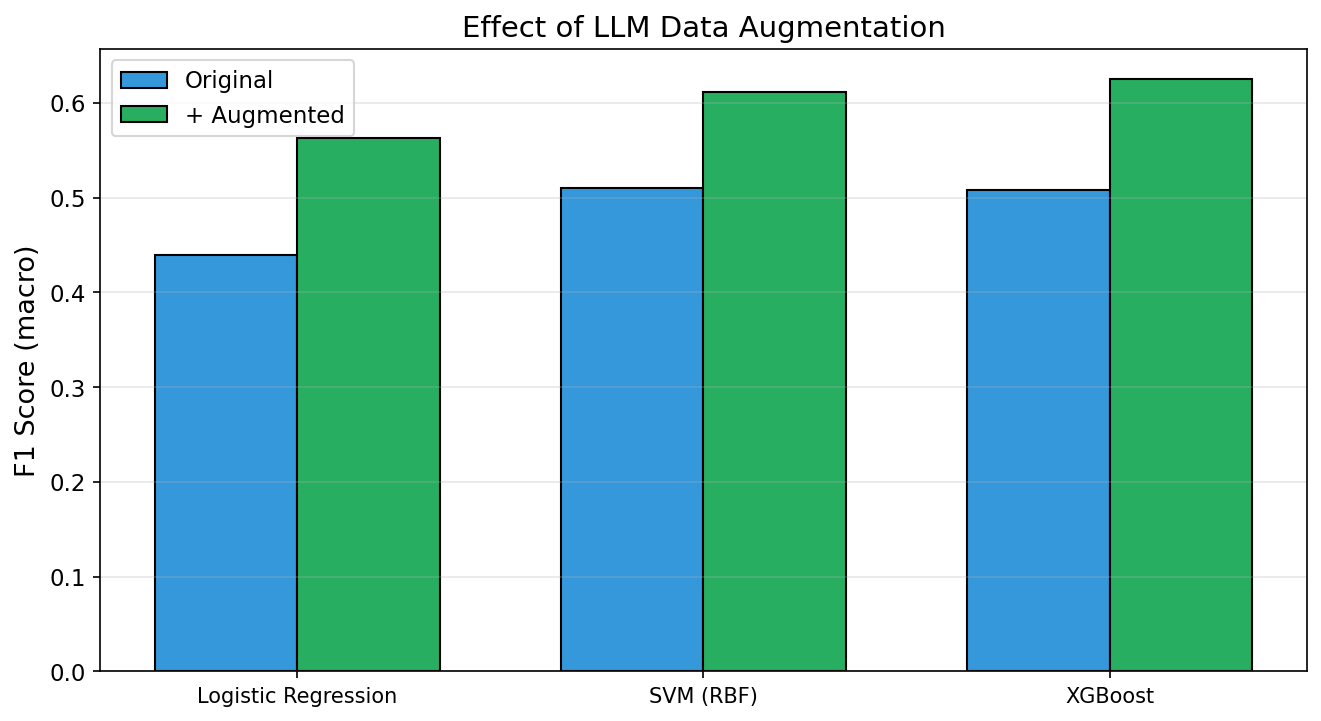
\includegraphics[width=0.6\linewidth]{figures/fig_augmentation_comparison.png}
    \caption{F1 score comparison with and without LLM data augmentation.}
    \label{fig:augment}
\end{figure}

The improvements are striking: all three models gain 10--12 F1 points,
with LR benefiting most (+12.4\%). These gains far exceed those from
SMOTE or PCA, indicating that the bottleneck was not feature engineering
or imbalance, but rather the quantity and diversity of labeled training
text. The LLM-generated rewrites expose the classifiers to a broader
range of syntactic phrasings for each class label, reducing overfitting
to specific lexical patterns in the original 1{,}129 samples.

% ─────────────────────────────────────────────────────────────────────────────
\section{Discussion}
\label{sec:discussion}
% ─────────────────────────────────────────────────────────────────────────────

\subsection{Expected vs.\ Observed Results}

Contrary to expectation, 21 handcrafted features outperformed 500
TF-IDF features for Logistic Regression and matched SVM, illustrating
that \emph{fewer, higher-quality features often outperform many noisy
ones} when data is limited. DistilBERT's advantage over the best
classical model (F1 = 0.580 vs.\ 0.542) was expected but modest, as
LLM-generated label noise constrains all methods equally. The most
surprising result was the magnitude of the augmentation gain
(+10--12 F1 points), confirming that data quantity---not model
capacity---is the primary bottleneck.

\subsection{Factors Affecting Performance}

\paragraph{Label noise.} LLM-generated zero-shot labels inevitably
contain systematic errors for ambiguous cases where evasiveness and
jargon overlap. Human annotation would improve absolute performance
but was infeasible at scale.

\paragraph{Class overlap.} \textsc{Evasive} and \textsc{Jargon} both
involve non-specific language, differing only in mechanism (hedging
vs.\ buzzwords), which explains their frequent confusion in all models.

\paragraph{Dataset size.} At $n = 1{,}129$, overfitting is a concern
for high-dimensional TF-IDF; PCA and augmentation both address this from
different angles (dimensionality reduction vs.\ data expansion).

\subsection{Key Takeaways}

\begin{enumerate}[nosep]
    \item \textbf{Domain features beat TF-IDF for linear models.}
          21 handcrafted features outperformed 500 TF-IDF features for LR,
          demonstrating the value of injecting domain knowledge.
    \item \textbf{PCA as regularization.} PCA-50 improved LR by 20\%,
          revealing that the baseline's weakness was overfitting, not
          insufficient model capacity.
    \item \textbf{Diagnose before fixing.} SMOTE had negligible impact
          (data already balanced); the real bottleneck was data quantity,
          confirmed by the 10--12 F1-point gains from augmentation.
    \item \textbf{Data is the dominant constraint.} LLM augmentation
          yielded the largest gains of any experiment---larger than
          architecture choice, feature engineering, or resampling.
\end{enumerate}

\subsection{Future Work}

Key next steps include: (1)~human annotation of a subset to calibrate
the LLM labeler; (2)~domain-specific models such as FinBERT with broader
hyperparameter search; (3)~expanding coverage to more companies and
fiscal years; and (4)~semi-supervised learning over the large pool of
unlabeled transcript text.

% ─────────────────────────────────────────────────────────────────────────────
% \section*{References}
% \addcontentsline{toc}{section}{References}
% ─────────────────────────────────────────────────────────────────────────────

\begin{thebibliography}{10}

\bibitem{sklearn}
F.~Pedregosa et al.,
``Scikit-learn: Machine learning in Python,''
\emph{Journal of Machine Learning Research}, vol.~12, pp.~2825--2830, 2011.

\bibitem{xgboost}
T.~Chen and C.~Guestrin,
``XGBoost: A scalable tree boosting system,''
in \emph{Proc.\ 22nd ACM SIGKDD}, pp.~785--794, 2016.

\bibitem{distilbert}
V.~Sanh, L.~Debut, J.~Chaumond, and T.~Wolf,
``DistilBERT, a distilled version of BERT: smaller, faster, cheaper and lighter,''
\emph{arXiv preprint arXiv:1910.01108}, 2019.

\bibitem{smote}
N.~V.~Chawla, K.~W.~Bowyer, L.~O.~Hall, and W.~P.~Kegelmeyer,
``SMOTE: Synthetic Minority Over-sampling Technique,''
\emph{Journal of Artificial Intelligence Research}, vol.~16, pp.~321--357, 2002.

\bibitem{seekingalpha}
SeekingAlpha,
``Earnings call transcripts,''
\url{https://seekingalpha.com}, accessed 2026.

\bibitem{qwen}
Qwen Team,
``Qwen3 Technical Report,''
Alibaba Cloud, \emph{arXiv preprint arXiv:2505.09388}, 2025.

\bibitem{tfidf}
G.~Salton and C.~Buckley,
``Term-weighting approaches in automatic text retrieval,''
\emph{Information Processing \& Management}, vol.~24, no.~5, pp.~513--523, 1988.

\bibitem{transformers}
T.~Wolf et al.,
``Transformers: State-of-the-art natural language processing,''
in \emph{Proc.\ EMNLP 2020: System Demonstrations}, pp.~38--45, 2020.

\end{thebibliography}

% ─────────────────────────────────────────────────────────────────────────────
% APPENDIX — Program Code
% (Does not count toward the 10-page limit)
% ─────────────────────────────────────────────────────────────────────────────
\clearpage
\appendix
\section*{Appendix: Program Code}
\addcontentsline{toc}{section}{Appendix: Program Code}

The pipeline consists of six scripts executed in order:

\begin{itemize}
    \item 01\_crawl\_transcripts.py
    \item 02\_extract\_qa\_pairs.py
    \item 03\_llm\_annotate.py
    \item 04\_build\_dataset.py
    \item 05\_experiments.py
    \item 06\_augment\_data.py
\end{itemize}

% \texttt{01\_crawl\_transcripts.py} $\to$
% \texttt{02\_extract\_qa\_pairs.py} $\to$
% \texttt{03\_llm\_annotate.py} $\to$
% \texttt{04\_build\_dataset.py} $\to$
% \texttt{05\_experiments.py} $\to$
% \texttt{06\_augment\_data.py}.

Selected key components from each script are shown below.
Full source is available at \url{https://github.com/weilin1205/CorporateEvasionDecoder}.

% ── Script 1: Transcript Crawling ────────────────────────────────────────────
\subsection*{Script 1: \texttt{01\_crawl\_transcripts.py} — Transcript Crawling}

This script fetches earnings call transcripts from SeekingAlpha via RapidAPI,
with retry logic and an API call budget cap.

\begin{lstlisting}[language=Python, basicstyle=\ttfamily\footnotesize,
    breaklines=true, frame=single, numbers=left, numberstyle=\tiny,
    caption={API request helper with retry and call-count enforcement.}]
MAX_API_CALLS = 480   # hard cap to avoid exceeding quota

def api_get(path: str, retries: int = 3) -> dict:
    """Send a GET request to the SeekingAlpha RapidAPI endpoint.
    Retries up to `retries` times with exponential back-off on failure.
    Raises RuntimeError if the global API call budget is exhausted."""
    global api_call_count
    if api_call_count >= MAX_API_CALLS:
        raise RuntimeError(f"API call limit reached ({MAX_API_CALLS})")
    for attempt in range(retries):
        try:
            conn = http.client.HTTPSConnection(RAPIDAPI_HOST)
            conn.request("GET", path, headers=HEADERS)
            res = conn.getresponse()
            raw = res.read()
            conn.close()
            api_call_count += 1
            decoded = raw.decode("utf-8").strip()
            if not decoded:
                raise ValueError(f"Empty response (HTTP {res.status})")
            return json.loads(decoded)
        except (json.JSONDecodeError, ValueError) as exc:
            wait = 2 ** (attempt + 1)      # 2s, 4s, 8s
            time.sleep(wait)
    return {}
\end{lstlisting}

\begin{lstlisting}[language=Python, basicstyle=\ttfamily\footnotesize,
    breaklines=true, frame=single, numbers=left, numberstyle=\tiny,
    caption={Main crawl loop: filter earnings calls and save raw JSON.}]
def crawl_all():
    df = pd.read_csv(TICKERS_PATH)
    for _, row in df.iterrows():
        ticker = row["Ticker"]
        items = get_transcript_list(ticker)

        # Keep only earnings-related transcripts by title keywords
        earnings = [
            x for x in items
            if x.get("type") == "transcript"
            and any(kw in (x.get("attributes") or {}).get("title", "").lower()
                    for kw in ["earnings call", "earnings conference",
                               "quarterly results", "financial results"])
        ]

        for item in earnings[:TRANSCRIPTS_PER_TICKER]:
            details  = get_transcript_details(str(item["id"]))
            html     = details["data"]["attributes"].get("content", "")
            # Convert HTML to plain text for downstream processing
            content_text = extract_text_from_html(html) if html else ""
            record = {
                "id": str(item["id"]), "ticker": ticker,
                "content_text": content_text, "content_html": html,
            }
            # Persist raw record; later scripts read from this directory
            with open(out_path, "w", encoding="utf-8") as f:
                json.dump(record, f, indent=2, ensure_ascii=False)
\end{lstlisting}

% ── Script 2: Q&A Extraction ─────────────────────────────────────────────────
\subsection*{Script 2: \texttt{02\_extract\_qa\_pairs.py} — Q\&A Pair Extraction}

Speaker turns are classified as \emph{analyst} or \emph{executive};
consecutive analyst turns are paired with the following executive response.

\begin{lstlisting}[language=Python, basicstyle=\ttfamily\footnotesize,
    breaklines=true, frame=single, numbers=left, numberstyle=\tiny,
    caption={Pairing analyst questions with executive answers.}]
def pair_qa_segments(segments, exec_names, analyst_names, record) -> list[dict]:
    """Scan speaker-turn segments and emit (question, answer) pairs.
    Skips operator turns; merges consecutive same-analyst turns into
    one question block; collects all subsequent executive turns as the answer."""
    pairs = []
    i = 0
    while i < len(segments):
        seg = segments[i]
        role = classify_speaker(seg["speaker"], exec_names, analyst_names)

        if role == "operator":           # skip queue/transition messages
            i += 1; continue

        if role == "analyst":
            question_parts = [seg["text"]]
            j = i + 1
            # Merge follow-up turns from the same analyst
            while j < len(segments):
                r = classify_speaker(segments[j]["speaker"],
                                     exec_names, analyst_names)
                if r == "analyst" and segments[j]["speaker"] == seg["speaker"]:
                    question_parts.append(segments[j]["text"]); j += 1
                else:
                    break

            # Collect the executive answer (may span multiple turns)
            answer_parts = []
            while j < len(segments):
                r = classify_speaker(segments[j]["speaker"],
                                     exec_names, analyst_names)
                if r in ("executive", "unknown"):
                    answer_parts.append(segments[j]["text"]); j += 1
                elif r in ("operator", "analyst"):
                    break
                else:
                    j += 1

            q = " ".join(question_parts)
            a = " ".join(answer_parts)
            # Quality filter: require minimum token lengths
            if len(q.split()) >= 8 and len(a.split()) >= 15:
                pairs.append({"question": q, "answer": a,
                              "ticker": record.get("ticker", ""),
                              "publish_date": record.get("publishOn", "")})
            i = j
        else:
            i += 1
    return pairs
\end{lstlisting}

% ── Script 3: LLM Annotation ─────────────────────────────────────────────────
\subsection*{Script 3: \texttt{03\_llm\_annotate.py} — LLM Annotation}

Each Q\&A pair is classified by a locally-run Qwen3.5-9B using a zero-shot
system prompt with explicit label criteria.

\begin{lstlisting}[language=Python, basicstyle=\ttfamily\footnotesize,
    breaklines=true, frame=single, numbers=left, numberstyle=\tiny,
    caption={Zero-shot annotation prompt and label extraction.}]
# System prompt defines labeling criteria unambiguously
SYSTEM_PROMPT = (
    "Classify the executive's earnings-call response as exactly one of: "
    "DIRECT, EVASIVE, or JARGON. Output ONLY that single word, nothing else.\n\n"
    "DIRECT  = specific numbers, facts, or clear explanations that address "
    "the question.\n"
    "EVASIVE = deflects, redirects, gives a non-answer, or avoids the "
    "question.\n"
    "JARGON  = excessive buzzwords or vague corporate language hiding lack "
    "of substance."
)

def parse_label(raw: str) -> int:
    """Extract integer label (0/1/2) from raw model output.
    Handles Qwen3 thinking-block artifacts and partial matches."""
    text = strip_thinking(raw).upper().strip()  # remove <think>...</think>
    first_word = re.sub(r"[^A-Z]", "", text.split()[0]) if text.split() else ""
    if first_word in LABEL_MAP:           # clean single-word output
        return LABEL_MAP[first_word]
    for label_name, label_id in LABEL_MAP.items():  # substring fallback
        if label_name in text:
            return label_id
    return -1   # unparseable; row will be dropped
\end{lstlisting}

% ── Script 4: Feature Engineering ────────────────────────────────────────────
\subsection*{Script 4: \texttt{04\_build\_dataset.py} — Feature Engineering}

The 21 handcrafted features are computed per Q\&A pair; TF-IDF is fit on
all answer texts. The two feature families are then concatenated.

\begin{lstlisting}[language=Python, basicstyle=\ttfamily\footnotesize,
    breaklines=true, frame=single, numbers=left, numberstyle=\tiny,
    caption={Handcrafted linguistic feature extraction (key dimensions).}]
def extract_handcrafted_features(question: str, answer: str) -> dict:
    """Return a dict of 21 scalar features capturing length, hedging,
    jargon density, numeric specificity, pronoun usage, and Q-A similarity."""
    q_words = question.lower().split()
    a_words  = answer.lower().split()
    a_sents  = [s for s in re.split(r"[.!?]+", answer) if s.strip()]
    a_len = max(len(a_words), 1)

    # --- Hedging: words that soften commitment (might, could, possibly, ...) ---
    hedge_count = sum(1 for w in a_words if w in HEDGE_WORDS)

    # --- Jargon: corporate buzzwords (synergy, leverage, ecosystem, ...) ------
    jargon_count = sum(1 for w in a_words if w in JARGON_WORDS)

    # --- Specificity: numeric tokens and domain metric phrases ----------------
    number_count = sum(1 for w in a_words if re.match(r"[\d$%,.]+$", w))
    metric_count = sum(1 for w in a_words if w in CONCRETE_METRICS)

    # --- Structure: does the answer open with a direct yes/no/number? ---------
    first_10 = " ".join(a_words[:10])
    starts_direct = int(any(first_10.startswith(s) for s in DIRECT_STARTERS))

    # --- Semantic overlap: Jaccard similarity of content words ----------------
    q_cw = {w for w in q_words if len(w) > 3}
    a_cw = {w for w in a_words if len(w) > 3}
    keyword_overlap = len(q_cw & a_cw) / max(len(q_cw), 1)

    return {
        "answer_word_count":   a_len,
        "avg_sent_length":     a_len / max(len(a_sents), 1),
        "qa_length_ratio":     a_len / max(len(q_words), 1),
        "hedge_word_ratio":    hedge_count / a_len,
        "jargon_word_ratio":   jargon_count / a_len,
        "number_ratio":        number_count / a_len,
        "metric_ratio":        metric_count / a_len,
        "first_person_ratio":  sum(1 for w in a_words
                                   if w in {"i","we","our","us","my"}) / a_len,
        "avg_word_length":     np.mean([len(w) for w in a_words]),
        "starts_with_direct_answer": starts_direct,
        "question_keyword_overlap":  keyword_overlap,
        # ... (10 additional ratio/count features follow the same pattern)
    }
\end{lstlisting}

\begin{lstlisting}[language=Python, basicstyle=\ttfamily\footnotesize,
    breaklines=true, frame=single, numbers=left, numberstyle=\tiny,
    caption={Combining TF-IDF and handcrafted features into one sparse matrix.}]
# TF-IDF on answer text: 500 features, unigrams + bigrams
tfidf = TfidfVectorizer(max_features=500, stop_words="english",
                        ngram_range=(1, 2), min_df=2, max_df=0.95)
X_tfidf = tfidf.fit_transform(df["answer"].fillna(""))  # sparse (n, 500)

# Q-A cosine similarity as a single additional feature
tfidf_qa = TfidfVectorizer(max_features=5000, stop_words="english")
tfidf_qa.fit(df["question"].tolist() + df["answer"].tolist())
Q_vecs = tfidf_qa.transform(df["question"].fillna(""))
A_vecs = tfidf_qa.transform(df["answer"].fillna(""))
qa_sim = np.array([cosine_similarity(Q_vecs[i], A_vecs[i])[0, 0]
                   for i in range(len(df))]).reshape(-1, 1)

# Stack: [TF-IDF (500) | handcrafted (20) | qa_similarity (1)] = 521 dims
X_combined = sparse.hstack([X_tfidf,
                             sparse.csr_matrix(
                                 np.hstack([X_handcrafted, qa_sim]))])
\end{lstlisting}

% ── Script 5: Experiments ─────────────────────────────────────────────────────
\subsection*{Script 5: \texttt{05\_experiments.py} — ML Experiments}

All classical models share a common \texttt{StandardScaler + Classifier}
pipeline evaluated with stratified 5-fold cross-validation.

\begin{lstlisting}[language=Python, basicstyle=\ttfamily\footnotesize,
    breaklines=true, frame=single, numbers=left, numberstyle=\tiny,
    caption={Baseline cross-validation loop for classical models.}]
def get_models():
    """Return the three classical classifiers with fixed hyperparameters."""
    return {
        "Logistic Regression": LogisticRegression(
            C=1.0, max_iter=2000, solver="lbfgs",
            multi_class="multinomial", random_state=42),
        "SVM (RBF)": SVC(
            C=1.0, kernel="rbf", probability=True, random_state=42),
        "XGBoost": XGBClassifier(
            n_estimators=100, max_depth=4, learning_rate=0.1,
            eval_metric="mlogloss", random_state=42, n_jobs=-1),
    }

def exp_baseline(X, y):
    skf = StratifiedKFold(n_splits=5, shuffle=True, random_state=42)
    scoring = {"accuracy": "accuracy",
               "f1_macro": make_scorer(f1_score, average="macro")}

    for name, model in get_models().items():
        # Pipeline ensures the scaler is re-fit inside each fold
        pipe = Pipeline([("scaler", StandardScaler(with_mean=False)),
                         ("clf", model)])
        cv = cross_validate(pipe, X, y, cv=skf,
                            scoring=scoring, return_train_score=True)
        print(f"{name}: Acc={cv['test_accuracy'].mean():.4f} "
              f"F1={cv['test_f1_macro'].mean():.4f}")
\end{lstlisting}

\begin{lstlisting}[language=Python, basicstyle=\ttfamily\footnotesize,
    breaklines=true, frame=single, numbers=left, numberstyle=\tiny,
    caption={PCA dimensionality reduction experiment across component counts.}]
def exp_pca(X, y):
    """Evaluate each model at multiple PCA component counts (25/50/100/200/full)
    to diagnose overfitting in high-dimensional feature space."""
    skf = StratifiedKFold(n_splits=5, shuffle=True, random_state=42)
    for nc in [25, 50, 100, 200]:
        for name, model in get_models().items():
            # PCA is placed inside the pipeline so it never sees test-fold data
            pipe = Pipeline([
                ("scaler", StandardScaler(with_mean=False)),
                ("pca",    PCA(n_components=nc, random_state=42)),
                ("clf",    model),
            ])
            s = cross_validate(pipe, X, y, cv=skf,
                               scoring={"f1": make_scorer(f1_score,
                                                          average="macro")})
            print(f"PCA-{nc} | {name}: F1={s['test_f1'].mean():.4f}")
\end{lstlisting}

\begin{lstlisting}[language=Python, basicstyle=\ttfamily\footnotesize,
    breaklines=true, frame=single, numbers=left, numberstyle=\tiny,
    caption={DistilBERT fine-tuning with early stopping (simplified).}]
# Key training settings
NUM_EPOCHS, LR, BATCH_SIZE = 10, 5e-5, 16
loss_fn = torch.nn.CrossEntropyLoss(weight=class_weights.to(device))

for epoch in range(NUM_EPOCHS):
    model.train()
    for batch_inputs, batch_labels in train_loader:
        outputs = model(**{k: v.to(device) for k, v in batch_inputs.items()})
        loss    = loss_fn(outputs.logits, batch_labels.to(device))
        loss.backward()
        torch.nn.utils.clip_grad_norm_(model.parameters(), 1.0)
        optimizer.step(); scheduler.step(); optimizer.zero_grad()

    # Early stopping: track best validation F1 across epochs
    val_f1 = evaluate_f1(model, test_loader, device)
    if val_f1 > best_val_f1:
        best_val_f1 = val_f1
        best_state  = {k: v.cpu().clone()
                       for k, v in model.state_dict().items()}
        patience_counter = 0
    else:
        patience_counter += 1
        if patience_counter >= 3:   # patience = 3
            break                   # restore best checkpoint after loop
\end{lstlisting}

% ── Script 6: Data Augmentation ───────────────────────────────────────────────
\subsection*{Script 6: \texttt{06\_augment\_data.py} — LLM Data Augmentation}

New training samples are generated by prompting Qwen3.5-9B to rewrite
\textsc{Evasive} answers as \textsc{Direct} and vice versa.

\begin{lstlisting}[language=Python, basicstyle=\ttfamily\footnotesize,
    breaklines=true, frame=single, numbers=left, numberstyle=\tiny,
    caption={Rewrite prompts and generation call for data augmentation.}]
# Prompt template for EVASIVE → DIRECT rewriting
REWRITE_EVASIVE_TO_DIRECT = """\
You are an expert corporate communication editor. Below is an analyst \
question and an evasive executive response. Rewrite ONLY the executive's \
response to be DIRECT: address the question head-on with specific, concrete \
information. Keep the same topic and approximate length.
Output ONLY the rewritten response, nothing else.

Question: {question}
Evasive Response: {answer}
Direct Rewrite:"""

def generate_rewrite(prompt_text: str) -> str:
    """Run the LLM and return the rewritten answer, stripping any
    Qwen3 chain-of-thought <think> blocks from the output."""
    inputs = tokenizer(prompt_text, return_tensors="pt",
                       truncation=True, max_length=4096).to(model.device)
    with torch.no_grad():
        output_ids = model.generate(**inputs, max_new_tokens=512,
                                    temperature=0.5, do_sample=True)
    new_tokens = output_ids[0][inputs["input_ids"].shape[1]:]
    raw = tokenizer.decode(new_tokens, skip_special_tokens=True)
    return strip_thinking(raw)   # removes <redacted_thinking>...</> blocks

def is_valid_rewrite(text: str) -> bool:
    """Reject outputs that leaked prompt text, reasoning scaffolding,
    or are too short to be a coherent executive response."""
    if len(text.split()) < 10: return False
    low = text.lower()
    if "you are an expert corporate communication editor" in low: return False
    if "redacted_thinking" in low: return False
    return True
\end{lstlisting}

\subsection*{Configuration: \texttt{config.py}}

\begin{lstlisting}[caption={Core configuration knobs.}]
# Centralized configuration for reproducibility
RAPIDAPI_HOST = "seeking-alpha.p.rapidapi.com"
MAX_API_CALLS = 480
TRANSCRIPTS_PER_TICKER = 8

LLM_MODEL_PATH = os.environ.get("Qwen/Qwen3.5-9B")
LLM_BATCH_SIZE = 1  # single-sample inference for reliability
LLM_MAX_NEW_TOKENS = 256  # room for thinking tags + label

CV_FOLDS = 5
RANDOM_STATE = 42
TFIDF_MAX_FEATURES = 500
PCA_COMPONENTS_LIST = [25, 50, 100, 200]
LEARNING_CURVE_FRACTIONS = [0.1, 0.2, 0.3, 0.4, 0.5, 0.6, 0.7, 0.8, 0.9, 1.0]
\end{lstlisting}

\end{document}
